\documentclass[12pt,a4paper]{scrartcl}
\usepackage[utf8]{inputenc}		% ermöglich die direkte Eingabe der Umlaute 
\usepackage[T1]{fontenc}		% das Trennen der Umlaute
\usepackage[ngerman]{babel}		% hiermit werden deutsche Bezeichnungen genutzt 
\usepackage{csquotes} 			% Gänsefüßchen nach gesetzter Sprache
\usepackage{graphicx}			% Bilder
\usepackage{subcaption}			% Für die Subfigures
\usepackage{geometry}			% Seitengröße
\usepackage[backend=biber,style=numeric,]{biblatex}	% Für das Literatursverzeichis
\usepackage{glossaries}			% Für Glossar
\usepackage{caption}			% Für schicke Titel bei Figures und Tabellen
\usepackage{chngcntr}			% Zähler für Figures und Tabellen anpassen
\usepackage{titling}			% Für schicke Titel
\usepackage{helvet}				% Für Helvetica 
\usepackage[onehalfspacing]{setspace}	% Seitenabstände
\usepackage{fancyhdr}			% Für die Kopf- und Fußzeile
\makeglossaries					% Glossar 
\counterwithin{figure}{section}	% Zähler
\counterwithin{table}{section}
\renewcommand{\familydefault}{\sfdefault}	% Auch wegen Font
\geometry{						% Seitengröße
  left=2.5cm,
  right=2.5cm,
  top=2.5cm,
  bottom=2cm,
  bindingoffset=5mm
}
\pagestyle{fancy}				% Stil setzen
\lhead{Containervirtualisierung}	% Header
\rhead{}\chead{}				% Andere Header leeren
\rfoot{Seite \thepage}
\lfoot{}\cfoot{}
\loadglsentries{glossary.bib}	% Datenfiles einfügen
\addbibresource{literatur.bib}

%------------------------
% Deckblatt Titel und co.
%------------------------

\pretitle{\begin{center}
\begin{figure}[h!]
	\begin{subfigure}{0.2\linewidth}
		
\includegraphics[scale=1]{DHBWLogo.png} 
	\end{subfigure}
	\hspace*{\fill}
	\begin{subfigure}{0.3\linewidth}
    	
\includegraphics[scale=0.25]{YellowMap.png}
	\end{subfigure}
\end{figure}
}
\posttitle{\end{center}}
\title{\Large{\bfseries Containervirtualisierung\\}\vspace{1cm}
	\large PRAXISBERICHT T1000\vspace{1cm}}
\author{
	\normalsize für die Prüfung zum\\
	\normalsize Bachelor of Science\\
	\normalsize des Studiengangs Informatik\\
	\normalsize Studienrichtung Informatik\\
	\normalsize an der\\
	\normalsize Dualen Hochschule Baden-Württemberg Karlsruhe\\\\
	\normalsize von\\
	\normalsize Jakob Jonathan Heitzmann
}
\date{\today}
\begin{document}

\maketitle
\vspace*{\fill}
\thispagestyle{empty}

%----------------
% Deckblatt unten
%----------------


\begin{tabular}{p{5cm}ll}
	Matrikelnummer & 9119328\\
	Kurs & TINF19B4\\
	Ausbildungsfirma & YellowMap AG, & Karlsruhe\\
	Betreuer & Markus Lind\\
	Prof. Jörn Eisenbiegler
\end{tabular}

\newpage

%--------------------------
% Eidesstattliche Erklärung
%--------------------------

\section*{Erklärung}
%TODO Titel ändern
(gemäß §5(3) der „Studien- und Prüfungsordnung DHBW Technik“ vom 29. 9. 2015)\\
Ich versichere hiermit, dass ich meine Projektarbeit mit dem Thema: ''Containervirtualisierung'' selbstständig verfasst und keine anderen als die angegebenen Quellen und Hilfsmittel benutzt habe. Ich versichere zudem, dass die eingereichte elektronische Fassung mit der gedruckten Fassung übereinstimmt.\\

\vspace*{2.5cm}

\begin{tabular}{lr}
\hline
\rule{0pt}{2ex}
Ort, Datum & Unterschrift
\\
\hspace{90mm} & \hspace{50mm} 
\end{tabular}
\newpage

\tableofcontents
\addcontentsline{toc}{section}{Inhaltsverzeichnis}
\newpage
\listoffigures
\addcontentsline{toc}{section}{Abbildungsverzeichnis}
\newpage
%\listoftables
%\addcontentsline{toc}{section}{Tabellenverzeichnis}
%\newpage
\printglossary
\addcontentsline{toc}{section}{Glossar}
\newpage

%-----------------------------------------------------------------------------------------------
%Hier beginnt das eigentliche Inhalt des Dokuments. (Davor nur Deckblatt bis Inhaltsverzeichniss)
%-----------------------------------------------------------------------------------------------

\section{Einführung}
Ziel der Arbeit ist es, vorzuzeigen, was ich in den ersten beiden Semestern meines Studiums bei der YellowMap AG gelernt und getan habe. Dabei wird sich auf die Gesamtheit der Bemühungen begrenzt, die dazu galten, die bestehende Serverstruktur zu brechen und einen Prototyp zu konzeptionieren, mit wessen Vorbild man das bestehende System in ein verteiltes System wandeln könnte. Zu diesem Zweck musste ich mich mit verschiedenen Arten der Serverkommunikation und Containervirtualisierung beschäftigen.

\subsection{Kontextuelle Betrachtung der Rahmenbedingungen}

YellowMap entwickelt und hostet in erster Linie Kartenanwendungen, bietet Entwicklern aber auch mit einer Java-Script-API die Möglichkeit, mit wenig Selbstaufwand selbst eine solche Anwendung zu entwickeln. Dabei laufen die Dienste mit allen gängigen großen Kartenanbietern so wie Google, OSM, Bing und sogar Baidu. Exemplarische Lösungen, die YellowMap anbietet, sind zum Beispiel die FilialFinder, mit denen alle Filialen eines Klienten auf dessen Webseite angezeigt werden können. Die Anzeige erfolgt natürlich auf einer Karte. Gesucht wird für gewöhnlich mit einer Umkreissuche auf den Standort des Gerätes. Die gefundenen Filialen können auch neben der Karte auch auf einer Liste sortiert ausgegeben werden.

\begin{figure}[h!]
	\centering
	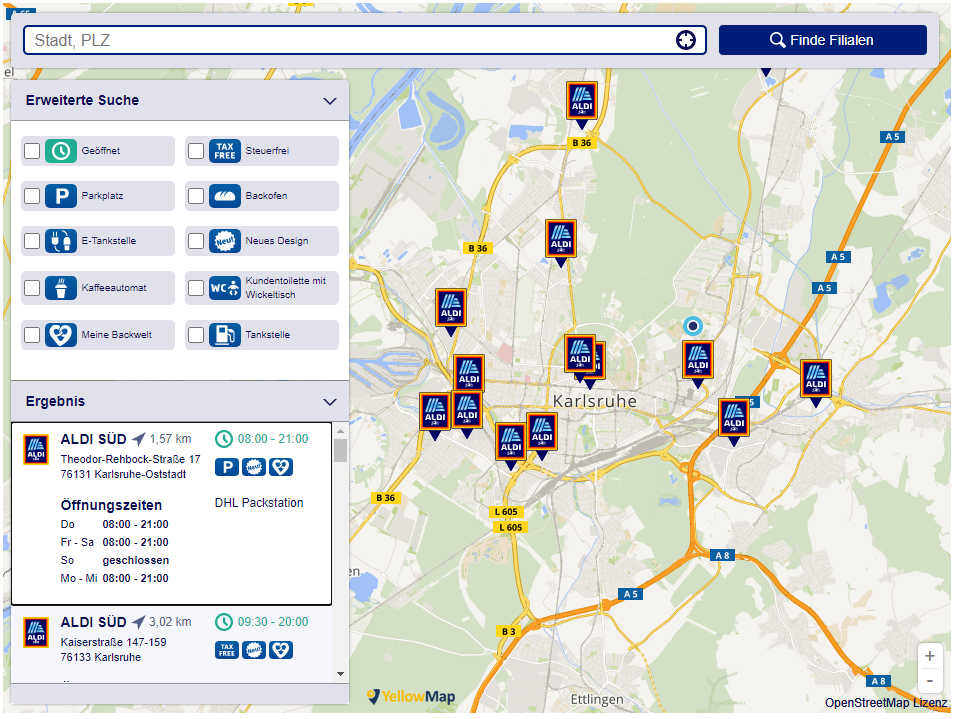
\includegraphics[scale=0.55]{YmFF.png}
	\caption[https://www.aldi-sued.de/filialen/ (Stand 28.08.2020)]{FilialFinder}
\end{figure}

%TODO Redo
%Zu Beginn bekam ich diverse Sonderaufgaben zugeteilt, die zu meiner Einarbeitung dienten. 
Im umrissenen Zeitraum habe ich viele Tätigkeiten besonders in den Bereichen Backend und Testing übernommen. Doch auch ein paar kleinere Aufgaben im Bereich Frontend fielen mir zu. Gearbeitet habe ich mit .NET Core, Gatling, HTML, CSS, JavaScript, Docker, Kubernetes und RabbitMQ. 
Darunter war die Entwicklung eines Dienstes, der dazu fähig ist, Termindaten von einer Datenbank zu ziehen und diese dann auf kleinen E-Paper-Bildschirmen anzuzeigen, was vollständig in C\# realisiert wurde. Auch entwickelte ich zu Demozwecken Testwebseiten, die Funktionen der JavaScript API präsentieren sollten. Ein anderes Projekt war die Realisierung von Stresstests auf ein schon bestehendes Projekt mittels Gatling. Dafür musste ich mich in die Programmiersprache Scala und Maven einarbeiten. 

Das Projekt, auf das ich in diesem Bericht näher eingehen möchte, war nun die Entwicklung eines Prototyps zur Containervirtualisierung und automatischen horizontalen Skalierung mittels Docker und Kubernetes, sowie die Entwicklung eines Prototyps für die Serverkommunikation mit Message Broker mittels RabbitMQ. Für diese Aufgabe wurden diese Technologien vorgegeben. 

\subsection{Das bisherige Serverdesign}
Das bestehende System wurde entworfen, damit viele Anwendungen unabhängig voneinander entwickelt werden können, ohne dass jede Funktionalität in jeder neuen Anwendung auch neu geschrieben werden müsste. Dazu greifen alle Projekte auf dieselbe Schnittstelle zu, diese bietet dann die einzelnen Funktionalitäten in einem einheitlichen Format. Diese Art der Kommunikation ermöglicht es, unabhängig von Art der Anwendung, die Anbindung an die internen Dienste sicherzustellen. 
Eine Anfrage eines Projekts auf diese Schnittstelle landet als Erstes am Proxy der \emph{Core}, also zu Deutsch dem Kern, hier wird die Anfrage angenommen und auf erster Ebene authentifiziert. Diese Anfrage wird dann an den \emph{System Call} weitergeleitet. Hier befindet sich der Partnerschalter. Er reichert die Daten der Anfrage mit den Daten zum gelieferten Partner aus der Datenbank an. Heißt er schaut zum Beispiel, von welchem Provider der Partner seine Daten beziehen möchte und trifft dem entsprechend Vorkehrungen, dass die Daten in den folgenden Aufrufen und Aktionen richtig weitergegeben und verarbeitet werden. Auch wird hier die auszuführende Aktion ermittelt und der dazugehörige Befehl in Form eines \emph{Commands} oder einer \emph{Command-Group}. 
Ein \emph{Command} reichert die Daten nun weiter an und reicht dann an einen Provider spezifische \emph{Command-Action} weiter, die die angefragte Aktion dann ausführt. In Abbildung 1.2 sehen wir einen Aufruf, der dann aber beispielshalber auf ein \emph{Lagacy-System} zugreift, das wiederum selbst eine eigene \emph{Command-Action} besitzt, die die Anfrage dann letztendlich ausführt. Diese \emph{Legacy-Systeme} werden aber in dieser Arbeit nicht weiter betrachtet, da diese nicht mehr aktiv weiterentwickelt werden.

\begin{figure}[h!]
	\centering
	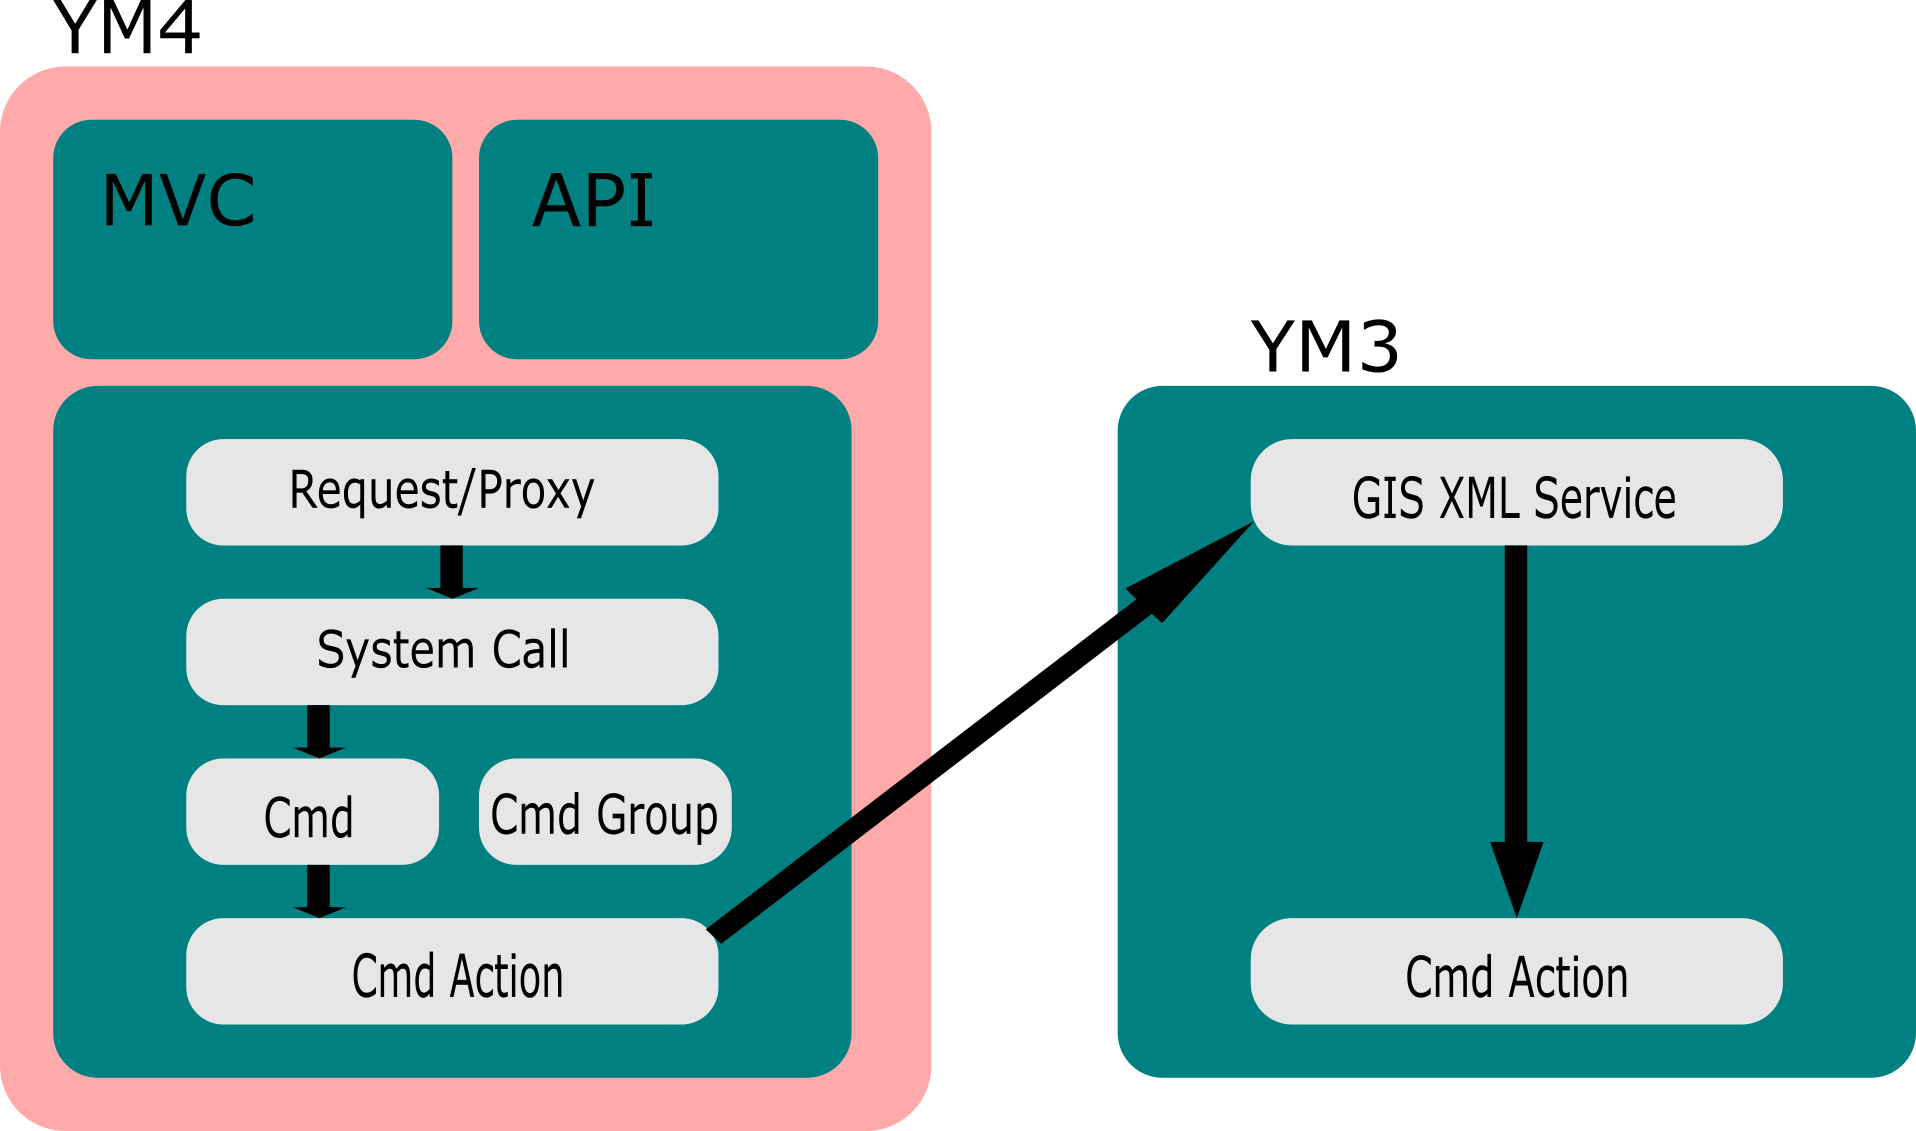
\includegraphics[scale=2]{YmSysReq.png}
	\caption[Selbst erstellte Grafik]{Beispielanfrage}
\end{figure}

Das System ist also kein Monolithisches, da es aus vielen Einzelprojekten besteht, die größtenteils unabhängig von einander agieren können, aber es ist ebenso kein verteiltes System, da sich trotz des modularen Designs alles auf demselben Server befindet.

\subsection{Ziel der Arbeit}
Beabsichtigt ist es, das eben beschriebene System nun in ein verteiltes System umzuwandeln. Ein verteiltes System ist ein System, dass aus einer Ansammlung von unabhängigen Komponenten besteht, die über ein Netzwerk miteinander kommunizieren, aber trotzdem nach außen als einzelnes System auftritt. Im Fall des Zielsystems soll dies mit einer zentralen API-Schnittstelle realisiert werden, die mögliche Anfragen dann an die verschiedenen Komponenten weiterleitet. So tritt es zwar als einzelnes System auf, aber kann komponentenweise sehr flexibel gehandhabt werden. So können einzelne Komponenten unabhängig vom Gesamtsystem einfach ausgetauscht werden. So wird uns auch ermöglicht, das System auf sehr spezifische Weise zu Skalieren.

Das Ziel meiner Arbeit liegt also darin, anhand der Entwicklung eines Prototyps die nötigen Grundlagen zu erarbeiten und mir das nötige Wissen anzueignen, das im Weiteren benötigt wird, um ein verteiltes System aufzusetzen und zu verwalten. Meine Arbeit legt den Grundstein für alle kommenden Projekte, die auf dieser Plattform entwickelt werden sollen und auf weitere Untersuchungen, die sich notwendigerweise aus dieser Untersuchung ergeben.

Wichtig für diesen Prototypen sind Flexibilität, Unabhängigkeit und Robustheit.

Das System soll aus austauschbaren Einzelkomponenten bestehen, die dynamisch miteinander kommunizieren. Dies bezeichnet die Flexibilität des Systems und stellt sicher, dass Komponenten in laufenden Betrieb ausgetauscht werden können und auch, dass der Ausfall einer Einzelkomponente innerhalb des Systems keinen Totalausfall für das gesamte System bedeuten würde.

Ebenso soll sollen die Komponenten in ihren eigenen Umgebungen unabhängig von den Anderen lauffähig sein, sodass bei der Entwicklung dieser Abhängigkeiten minimiert werden. So sollen weniger Konflikte zwischen verschiedenen Projekten und ihren Abhängigkeiten gewährleistet werden, was wiederum die Flexibilität erhöht, da dies das Aufrüsten einzelner Komponenten innerhalb des Systems ermöglicht.

Weiterhin soll das System auch Robustheit beweisen, indem es bei dem Ausfall von Komponenten innerhalb des Systems auf diesen reagieren und diese wieder neu starten sollte. Also muss das System sich selbst nicht nur überwachen, sondern auch regenerieren können. 

\newpage
\section{Serverkommunikation mit Message Broker} \label{rabbit}
Zuerst begann ich den Prototypen für die Serverkommunikation mittels Message Broker zu konzeptionieren. Der Message Broker sollte eine neue interne Schnittstelle zwischen dem Serversystem und dem \emph{Legacy-System} etablieren, da diese zuvor via normale \emph{HTTP}-Aufrufe, die über das externe Netz gingen, realisiert wurde. Dies benötigte das Herauslösen eigenständiger Komponenten des \emph{Legacy-Systems} und die Umwandlung dieser in sogenannte \emph{Microservices}. Im Hinblick auf die späteren Änderungen, die noch an dem System vorgenommen werden sollten, sollte auch die Möglichkeit betrachtet werden, die Protokollierung von Systemdaten über den Message Broker auf eine Vielzahl von Empfängersystemen zu ermöglichen.

\subsection{Funktion eines Message Brokers}
Ein Message Broker ist ein System zur Nachrichtenübertragung und Nachrichtenverteilung. Dafür fungiert der Message Broker selbst als der zentrale Umschlagplatz, von dem aus Nachrichten empfangen und verteilt werden. Ebenso übersetzt er aktiv zwischen verschiedenen Protokollen\cite{mesBro}. Er stellt eine Art \emph{Middleware} da, was bedeutet, dass er als neutrale Komponente im System nur für die Vermittlung von Information zwischen anderen Komponenten verantwortlich ist.

\subsection{Anwendungsspezifische Betrachtung}
In Hinblick auf die Containervirtualisierung ist das Prinzip eines Message Brokers mehr als nützlich.
Ein Message Broker kann einen Nachrichten-Pool schaffen, den er kontinuierlich und gezielt mit Nachrichten versorgt, die dann von den letztendlichen Verbrauchern konsumiert werden können. Dadurch schafft man ein Netz von Geräten, die nur noch eine zentrale Adresse kennen müssen und dadurch dynamischer und unabhängiger voneinander agieren können. 

\begin{figure}[h!]
	\centering
	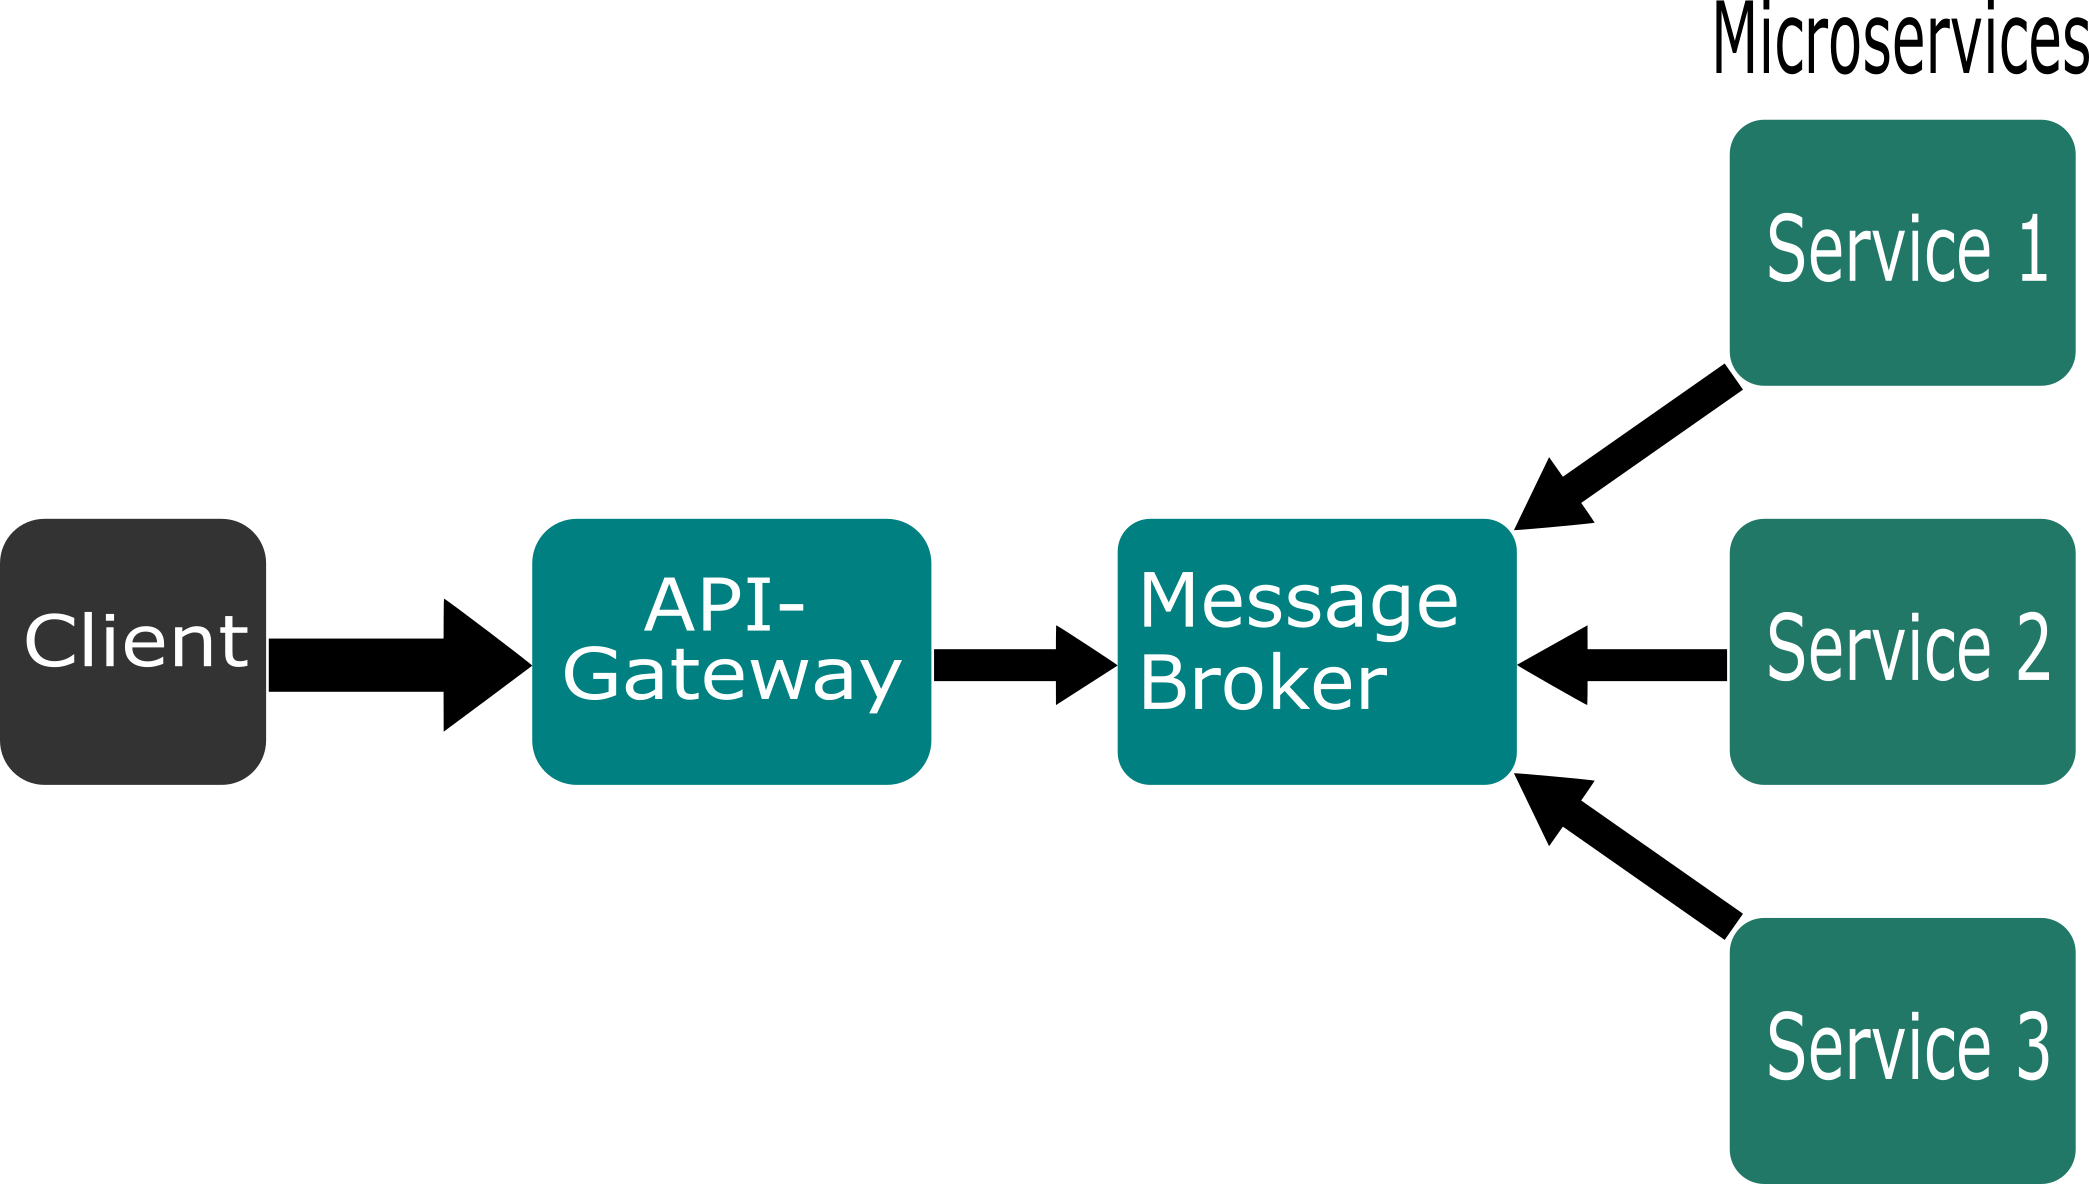
\includegraphics[scale=1.8]{MesBroSys.png}
	\caption[Selbst erstellte Grafik]{Serversystem mit Message Broker}
\end{figure}

In Abbildung 2.1 sehen wir, wie der Message Broker seine Funktion als \emph{Middleware} zwischen einem \emph{API-Gateway} und mehreren Diensten erfüllt.  

\subsection{RabbitMQ}
RabbitMQ ist ein Open-Source-Message-Broker, der das \emph{Advanced-Message-Queuing-Protokoll (AMQP)} unterstützt und sogar um einige nützliche Funktionalitäten erweitert\cite{rabExt}.
Darunter ist eine grafische Managementoberfläche und Unterstützung für \emph{Remote-Procedure-Calls (RPC)}. Dies sind beides Funktionen, die enorm praktisch für die vorgesehene Verwendung sind.

Mittels grafischer Managementoberfläche wird die Fehlersuche immens einfacher gestaltet. Sie zeigt an, an welchen Endpunkten Nachrichten eingetroffen sind, wie viele es sind, ob ein Endpunkt gemeldete Konsumenten hat und vieles mehr. Mit ihr kann man ebenfalls sämtliche Konstrukte selbst erzeugen und die Nachrichten im allgemeinen Verwalten. 

Ein \emph{RPC} ermöglicht es uns, eine Funktion auf einem anderen Gerät auszuführen und ebenso dessen Wert zurückgeliefert zu bekommen. Was genau das ist, was wir in einem verteilten System wollen.

\subsubsection{Grundlegende Funktionsweise}

RabbitMQ stellt in erster Linie einen Serverdienst, eine Managementoberfläche und Nutzerschnittstellen zur Verfügung. Der Serverdienst nimmt Nachrichten entgegen und Verwaltet diese. 
Er besitzt \emph{Exchanges} und \emph{Queues}. Ein \emph{Exchange} nimmt eine Nachricht entgegen und verteilt diese an eine oder mehrere \emph{Queues}, die ein \emph{Binding} auf den jeweiligen \emph{Exchange} haben. 

\begin{figure}[h!]
	\centering
	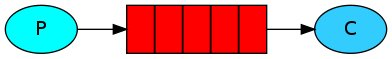
\includegraphics[scale=1]{P2C.jpg}
	\caption[https://www.rabbitmq.com/tutorials/tutorial-one-dotnet.html]{Produzent, Queue und Konsument}
\end{figure}

Es gibt verschiedene Arten von \emph{Exchanges}, die Nachrichten auf verschiedene Weise verteilen. 

Ein \emph{Fanout-Exchange} sendet die Nachricht an jede \emph{Queue}, mit der er ein \emph{Binding} besitzt. 

Ein \emph{Direct-Exchange} sendet eine Nachricht nur an eine \emph{Queue}, wenn der \emph{Routing-Key} der Nachricht mit dem Namen einer \emph{Queue} übereinstimmt, die natürlich auch ein \emph{Binding} auf dem \emph{Exchange} haben muss.

\begin{figure}[h!]
	\centering
	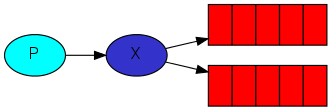
\includegraphics[scale=1.65]{exchanges.png}
	\caption[https://www.rabbitmq.com/tutorials/tutorial-three-dotnet.html]{Produzent, Exchange und Queue}
\end{figure}

Ein \emph{Topic-Exchange} wiederum verteilt an mehrere \emph{Queues} in seinem \emph{Binding}. Dabei dürfen die \emph{Queues} keinen willkürlichen Namen tragen, sondern müssen einem gewissen Namensmuster Folgen, dass teilweise den \emph{Routing-Key} der zu empfangenden Nachrichten reflektieren soll. Wenn zum Beispiel der \emph{Routing-Key} einer Nachricht \emph{core.failure.critical} wäre, so wäre auch \emph{*.*.critical} ein Name, unter dem eine \emph{Queue} diese Nachricht empfangen würde. Dabei steht das Sternchen als Platzhalter für jedes mögliche Wort. Die Punkte reflektieren die Punkte im \emph{Routing-Key}. Eine Raute ist dabei ein Platzhalter für mehrere Wörter, also über Punkte hinaus. 

Der \emph{Standard-Exchange} ist ein \emph{Direct-Exchange} und wird innerhalb des Codes mithilfe einer leeren Zeichenkette ausgewählt. Er ist auch notwendigerweise mit allen \emph{Queues} verbunden.

Ein \emph{Exchange} wird von Produzenten befüllt. Ein Produzent erzeugt Nachrichten und schickt diese an \emph{Exchanges} damit diese dann an einer oder mehreren \emph{Queues} konsumiert werden.

Eine \emph{Queue} ist ein Speicher, der Nachrichten zwischenspeichert und nach dem \emph{First-in-First-Out (FIFO)}-Prinzip an Konsumenten verteilt. Sie sind Anlaufstelle für Konsumenten. 

Ein Konsument meldet sich bei einer \emph{Queue} und wird dort in eine Liste von Konsumenten aufgenommen. So wird er dann von dem Server mit Nachrichten bedient. Wird eine Nachricht konsumiert, kann ein Konsument diesen Vorgang bestätigen, falls der Produzent es wünscht. Das heißt wiederum aber auch, dass der Produzent nun auch auf die Antwort des Konsumenten wartet und ihn somit potenziell blockiert.

Eine Nachricht wird in RabbitMQ mit vielen Attributen abgesendet. Sie folgt in erster Linie dem \emph{AMQP}, doch RabbitMQ hat diese um einige Funktionen erweitert. So kommt zum Beispiel das Attribut \emph{reply\_to} mit. In diesem Attribut kann eine Antwortadresse für zum Beispiel den Absender hinzugefügt werden. Dieses Attribut wird später im \emph{Remote-Procedure-Call} benutzt. Sonst kommt offensichtlicherweise Informationen über die Zieladresse und den \emph{Ziel-Exchange}, den \emph{Routing-Key} und natürlich auch die eigentliche Nachricht, dem \emph{Body}, mit.

Die Managementoberfläche und Nutzerschnittstellen bieten eine Plattform, von der man mit dem Serverdienst wie beschrieben interagieren kann.

\subsubsection{Remote-Procedure-Call (RPC)}
Der \emph{RPC} ist ein Muster, das uns ermöglicht, auf eine Nachricht eine entsprechende Antwort zu bekommen, wie bei einem Funktionsaufruf. 

\begin{figure}[h!]
	\centering
	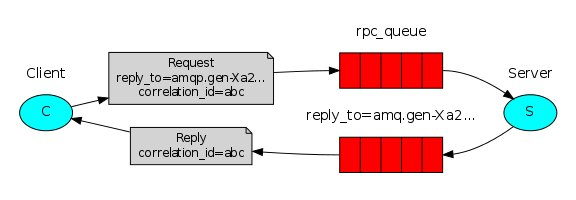
\includegraphics[scale=0.74]{RPC.jpg}
	\caption[https://www.rabbitmq.com/tutorials/tutorial-six-dotnet.html]{RPC}
\end{figure}

Für dieses Muster verwenden wir zuerst einen normalen Produzenten, den wir jedoch um die Attribute \emph{reply\_to} und \emph{correlation\_id} erweitern. Wir setzten die \emph{Antwort-Queue} auf einen zufälligen Namen, den wir uns von RabbitMQ generieren lassen. 
Die \emph{correlation\_id} lassen wir zufällig generieren. Dann öffnen wir einen Konsumenten auf eben diese \emph{Queue}.

Der Konsument nimmt nun ganz normal diese Nachricht an und ließt das \emph{reply\_to}-Attribut aus. Und sendet eine Antwort auf diese \emph{Queue}.

Der Sender konsumiert diese Antwort und überprüft die \emph{corelation\_id}. Wenn diese nun übereinstimmt, gibt er den Antworttext zurück und trennt die Verbindung zu der \emph{Queue}, die, wenn diese die Eigenschaft  \emph{auto\_delete} gesetzt hat, sich dann von alleine löscht.

\subsection{Implementierung}

Bevor ich beginnen konnte, meinen Prototypen zu bauen, musste ich eigenständige Teile in der Serverarchitektur erkennen und isolieren. 
Meine Methodik lässt sich darauf beschränken, dass ich das Projekt kopierte, die zu isolierende Funktion im Code ausmachte und nun alles entfernte, was offensichtlich keine Abhängigkeit zu der Funktion hatte. 
Nun konnte ich den Aufruf durch die alte Schnittstelle löschen und mit dem Aufruf durch RabbitMQ ersetzen. Ich benutzte dafür das  \emph{RPC}-Muster, das ich zuvor schon beschrieben habe. 

\begin{figure}[h!]
	\centering
	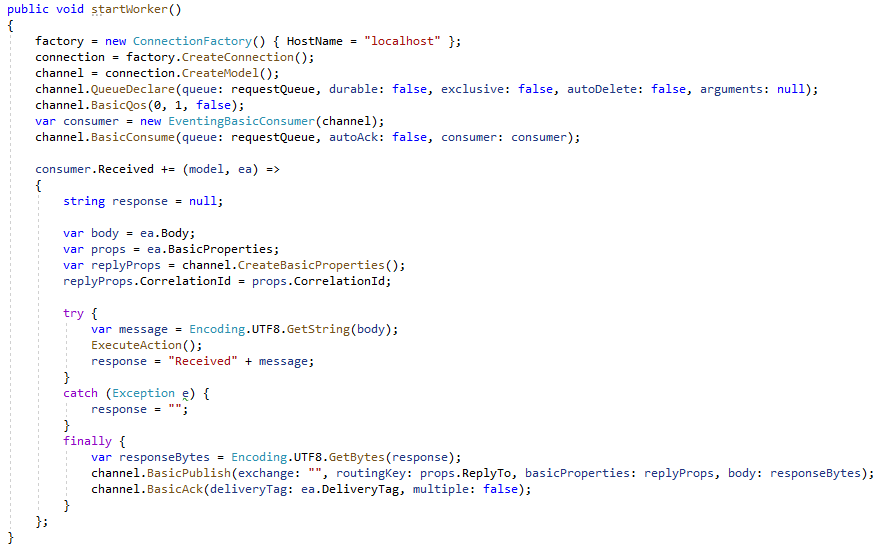
\includegraphics[scale=0.6]{RPCWorkerWhite.png}
	\caption[Screenshot]{RPC-Empfänger}
\end{figure}

In Abbildung 2.5 sehen wir ein Beispiel für einen Empfänger. Als Erstes wird eine Verbindung zum Server aufgebaut und die \emph{Anfrage-Queue} deklariert. Zusätzlich konfigurieren wir den Server nur eine unbestätigte Nachricht pro \emph{Queue} zu erlauben. Wird dieser Wert erreicht, so werden keine Nachrichten mehr von der \emph{Queue} verteilt. Dann wird ein Konsument erzeugt und dem Event \emph{Received} via \emph{Lambda}-Ausdruck eine Funktion übergeben, die auf empfangene Nachrichten reagiert. Innerhalb dieser wird die Nachricht ausgelesen und mit den ausgelesenen Informationen eine Methode aufgerufen. Daraufhin schickt sie die Rückgabe der Methode an die \emph{Antwort-Queue}. Zu guter Letzt wird der Konsument dann auch an die \emph{Anfrage-Queue} angehängt.

Den Sender oder auch \emph{RPC-Client} genannt, implementierte ich an der Stelle, an welcher auch normalerweise der \emph{HTTP}-Aufruf für eben diese Funktion stattfand.

\begin{figure}[h!]
	\centering
	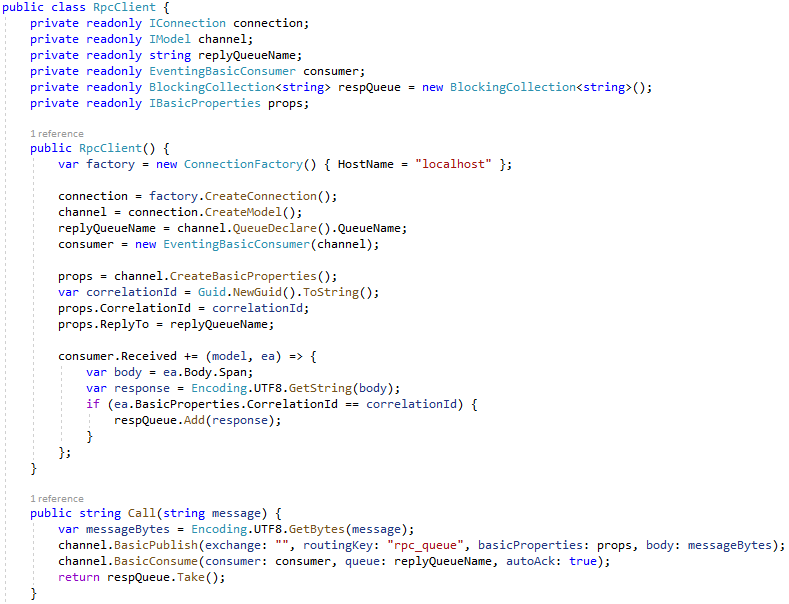
\includegraphics[scale=0.7]{RPCKlientWhite.png}
	\caption[Screenshot]{RPC-Sender}
\end{figure}

Abbildung 2.6 zeigt einen Beispiel-Sender. Er baut wie schon der Empfänger zuerst eine Verbindung zum Server auf. Danach erzeugt er Eigenschaften für die Nachricht und befüllt diese mit einem zuvor erzeugten Namen für die \emph{Antwort-Queue} und einer zufälligen \emph{correlation\_id}. Nun wird nur noch dem Konsumenten eine Funktion übergeben, die den Inhalt der Nachricht als Zeichenkette zwischenspeichert. Wenn nun die \emph{Call}-Methode aufgerufen wird, wird eine Nachricht an die \emph{Anfrage-Queue} gesendet und direkt danach der Konsument an die \emph{Antwort-Queue} angehängt. Wurde die Antwort empfangen, wird nun die zwischengespeicherte Zeichenkette zurückgegeben und aus dem Zwischenspeicher entfernt.

Nachdem ich also eine Methode hatte, Zeichenketten mit dem Message Broker austauschen zu können, musste ich nun entscheiden, wie ich die Übergabeobjekte in solch eine Zeichenkette umwandeln sollte, sodass diese auch am Empfänger rückübersetzt werden konnten.
Ich entschied mich dafür, die Objekte in eine \emph{JSON}-Zeichenkette umzuwandeln, da dies das Rückübersetzen in ein Objekt sehr einfach gestaltete und ich bis zu diesem Zeitpunkt aus den vorherigen Aufgaben schon mehrere Erfahrungen zum Umgang mit \emph{JSON}-Objekten hatte. 
Da es sich aber um komplexe Objekte handelte, die nicht nur Basisdatentypen als Werte hatten, musste ich den Übersetzer der \emph{JSON}-Bibliothek, die ich verwendete, anpassen, sodass innere Objekte der Anfrage mit übersetzt werden konnten. 
Dann machte ich mich langsam daran, gezielt überflüssigen Code zu entfernen, solange bis nur noch der Kern der Funktion über war.

Den Prototypen zum \emph{Fanout-Exchange} implementierte ich als \emph{Dead-Letter-Exchange}, eine Art \emph{Exchange}, den man bei der Initialisierung einer \emph{Queue} angeben kann. An ihn werden Nachrichten gesendet, wenn diese Nachrichten eine in der \emph{Queue} gesetzten \emph{Time-To-Live (TTL)} überschreiten.


\newpage
\section{Containervirtualisierung mit Docker} \label{docker}
Docker ist ein Werkzeug zur Erstellung und Verwaltung von Containern. 
Container sind kleine, voneinander unabhängige Umgebungen, in denen Programme lauffähig und von außerhalb gezielt erreichbar sind. Sie werden dafür eingesetzt, eine Anwendung von äußeren Einflüssen zu befreien. Ihre Prämisse lautet, wenn eine Anwendung auf einem System funktioniert, funktioniert sie auf allen Systemen. Ein Container hat für gewöhnlich nur das Nötigste installiert, um lauffähig zu sein, alles andere wird vom Entwickler selbst beigesteuert. Was ihnen wiederum einen entscheidenden Vorteil im Vergleich zu einer \emph{virtuellen Maschine (VM)} gibt. Aber nicht nur das. Einen Container aufzusetzen ist auch mit um einiges weniger Aufwand verbunden als das Aufsetzen einer \emph{VM}. 

In Hinsicht auf die gezielte Serverstruktur soll Docker das Rückgrat dieser stellen. Die einzelnen Funktionen sollen durch die Containervirtualisierung voneinander abgekoppelt und skalierbar werden.

\subsection{Grundlagen der Containervirtualisierung}

Auch wenn Containervirtualisierung eine Art der Virtualisierung ist, laufen hierbei die Container nicht über ein Gastbetriebssystem, sondern befinden sich trotzdem auf ihrem Hostbetriebsystem. Auch wenn sie strikt getrennte Programminstanzen mit allesamt eigenen Abhängigkeiten und Ressourcen sind, teilen sie sich denselben Systemkernel. 

\begin{figure}[h!]
\centering
	\begin{subfigure}{0.4\linewidth}
		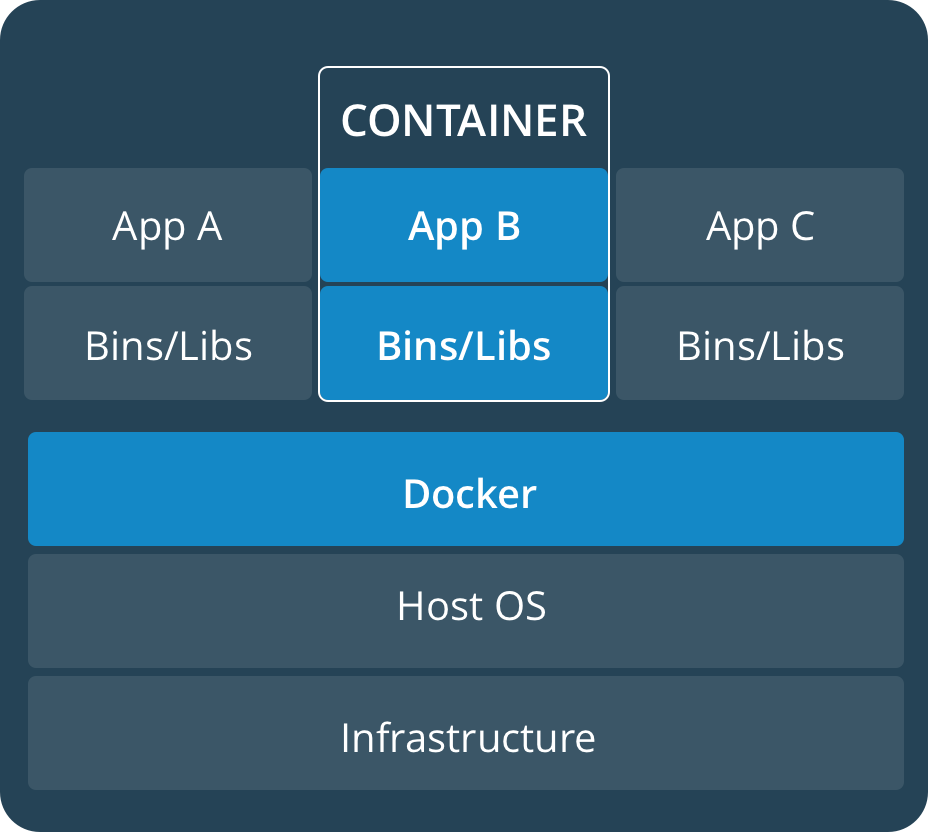
\includegraphics[scale=0.2]{DockerContainer.png} 
	\end{subfigure}
	\hspace*{1 cm}
	\begin{subfigure}{0.4\linewidth}
    	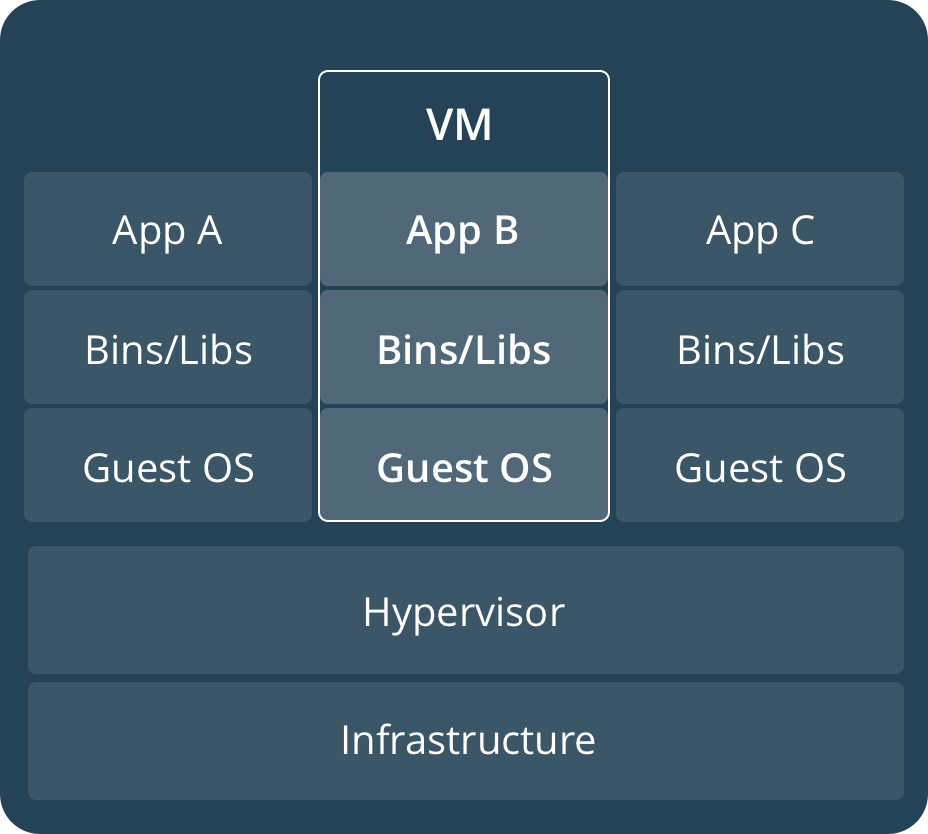
\includegraphics[scale=0.2]{DockerVM.png}
	\end{subfigure}
	\caption[https://docs.docker.com/get-started/]{Containervirtualisierung im Vergleich zu klassischer Virtualisierung.}
\end{figure}

Auf Abbildung 3.1 sehen wir die Containervirtualisierung im Vergleich zur klassischen Virtualisierung. Es ist leicht zu erkennen, dass durch die Einsparung des Gastbetriebssystems auf jeder Instanz wertvoller Speicherplatz erhalten werden kann. 

Dieser Vorteil wird aber erst bei einer größeren Anzahl an Instanzen richtig ersichtlich, weswegen diese Art der Virtualisierung bei verteilten Systemen zum Einsatz kommt. Ein verteiltes System ist ein System, in dem die einzelnen verschiedenen Funktionen, die das System erfüllt, von unabhängigen, getrennten Komponenten erfüllt werden, die auf eine dynamische Weise miteinander verbunden sind. So wird es ein Einfaches, dieses System horizontal zu Skalieren. Das heißt, Instanzen des zu Skalierenden hinzuzufügen. Durch die dynamische Einbindung aller Komponenten wird sicher gestellt, dass die Last nun auf alle Instanzen desselben Typs gleichmäßig verteilt sind. Dies geschieht zum Beispiel mit einem \emph{Load Balancer}. Mit einem Message Broker ist Ähnliches zu erreichen.

\subsection{Docker Grundlagen}

Docker ist nun eine Plattform, auf der wir mit Containern interagieren können. Das heißt unter anderem Container erzeugen und löschen, Ports teilen und Speicher zuteilen. Ein Container wird mit einem \emph{Image} erzeugt. Ein \emph{Image} ist ein Abbild der auszuführenden Programminstanz und wird aus einer \emph{Registry}, einer zentralen Sammelstelle für \emph{Images}, gezogen. Docker \emph{Images} werden mit \emph{Dockerfiles} erzeugt und können dann lokal verwaltet und auf externe \emph{Registries} geschoben werden. Eine \emph{Registry}, die nicht über \emph{HTTPS}, sondern nur über \emph{HTTP} erreichbar ist, nennt man eine \emph{Unsecure Registry} und muss der \emph{daemon.json} hinzugefügt werden. Das geht unter Windows einfach über die Einstellungen des Programms \emph{Docker Desktop}. Da mehrere Instanzen desselben Containers auch mehrere Anwendungen auf demselben Port und derselben Adresse heißen würde, muss man auf die Ports, die von der Anwendung verwendet werden, von anderen Ports verweisen. Dies nennt sich \emph{Port-Mapping}. 
Docker bietet auch Container mit Netzwerken zu verbinden, sodass ein \emph{Domain Name System (DNS)} Containernamen auf ihre IP-Adressen übersetzt. Es gibt zwar auch Standardlösungen für diese Netzwerke, auf denen aber die Auflösung von Containernamen nicht möglich ist. Deshalb ist es ratsam, diese Netzwerke selbst zu definieren.
Dabei ist aber zu bedenken, ob die Anfrage auch wirklich vom Container aus gesendet wird und nicht wie im Falle von JavaScript clientseitig gestellt wird.
Ein anderes Konzept, das Docker einführt, ist \emph{Volume}. Ein \emph{Volume} ist eine Art Speicher, mit dem sich Container verbinden und es dann benutzen können.
Container können über die Kommandozeile mit dem Befehl  \emph{docker run example/image:test} gestartet werden. Dabei können zahlreiche Parameter mitgegeben werden. Mit \emph{-p} können so \emph{Port-Mappings} erstellt werden. Die lokalen \emph{Images} können mit \emph{docker images} eingesehen werden. Mit \emph{docker ps} werden die laufenden Container angezeigt. Möchten wir auch die beendeten Container aufgelistet haben, so fügen wir das Kürzel \emph{-a} an. Wenn ein Container gestoppt werden soll, geht dies mit \emph{docker stop container\_id} und zum Entfernen mit \emph{docker rm container\_id}. \emph{Images} werden mit \emph{docker rmi image\_id} entfernt. Zur Fehlersuche können wir mit \emph{docker logs container-name} auf die \emph{Log}-Dateien eines Containers zugreifen.

\begin{figure}[h!]
	\centering
	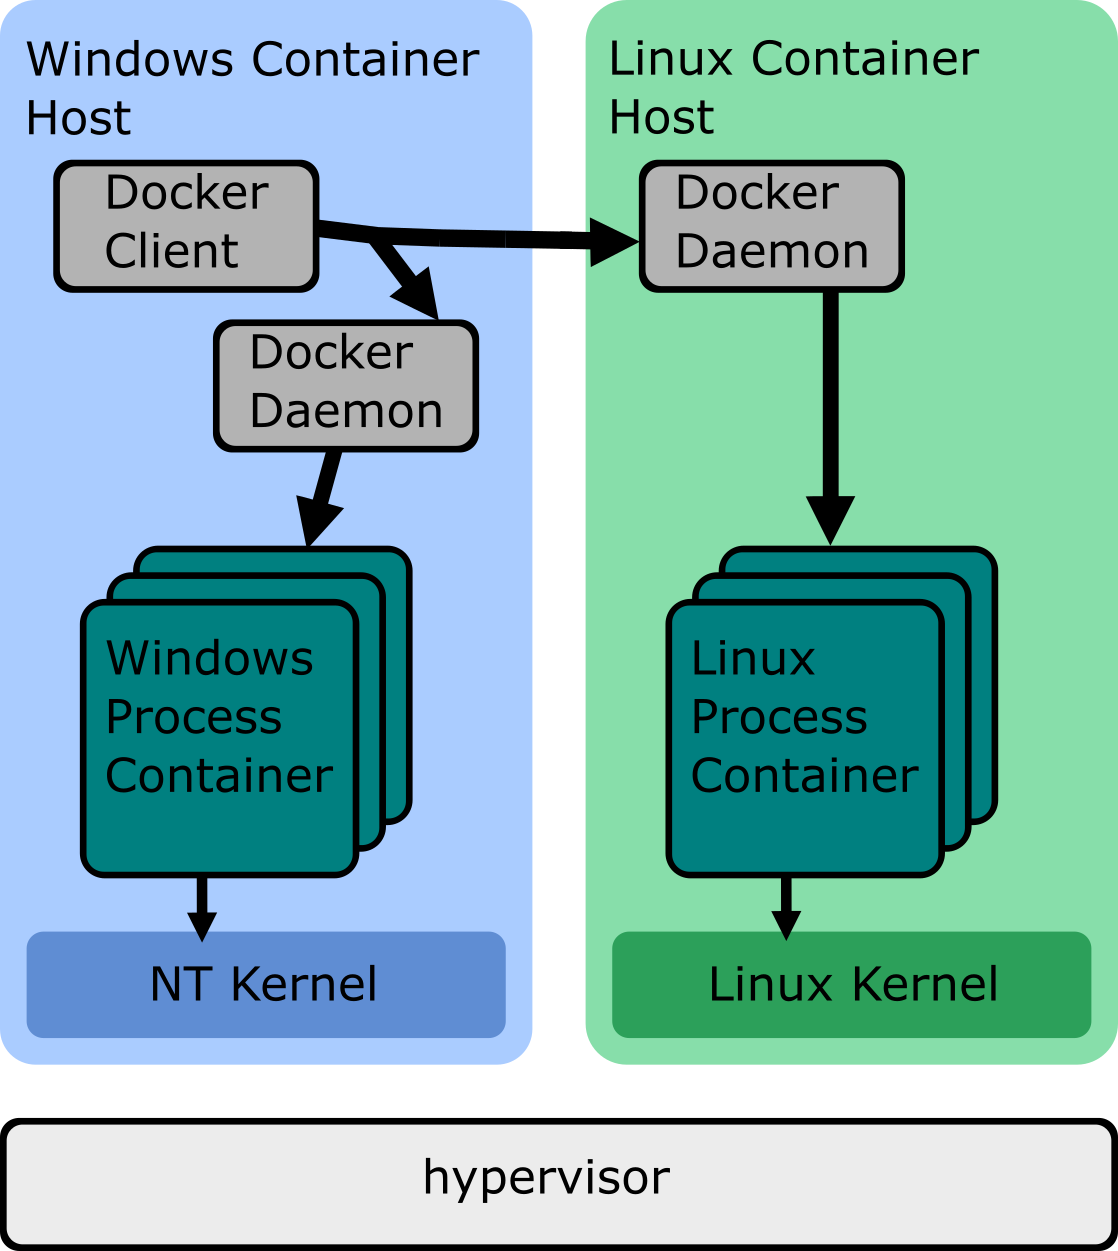
\includegraphics[scale=2]{DockerWindows.png}
	\caption[https://docs.microsoft.com/de-de/virtualization/windowscontainers/deploy-containers/linux-containers]{Linux Container auf Windows}
\end{figure}

Für gewöhnlich werden Linux-Container verwendet, auch unter Windows. Docker erstellt dafür dann eine \emph{VM}, die das gewünschte Hostbetriebssystem so zur Verfügung stellt. Das wird auf Abbildung 3.2 verdeutlicht. 

\subsubsection{Dockerfile}

Wie schon zuvor erwähnt wird mit einem \emph{Dockerfile} ein Image unserer Anwendung erstellt. 

\begin{figure}[h!]
	\centering
	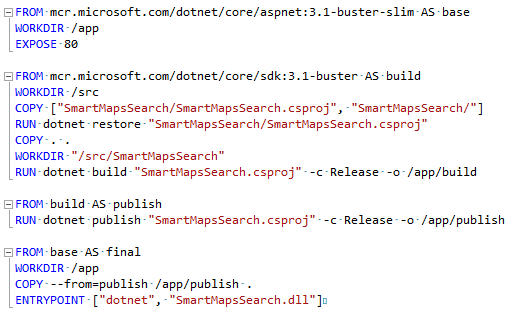
\includegraphics[scale=1]{DockerfileWhite.png}
	\caption[Screenshot]{Beispiel für einen Dockerfile}
\end{figure}

In Abbildung 3.3 sehen wir, wie ein \emph{Dockerfile} exemplarisch aussehen könnte. Als Erstes wird eine Basis referenziert, die unser \emph{Image} braucht, um ausgeführt werden zu können. In diesem Fall ist dies \emph{.Net Core 3.1}. Danach geben wir die Anweisung, den Port 80 für diese Anwendung freizugeben. Nun wird alles Programmrelevante in den Kontext gezogen, gebaut und veröffentlicht. Zuletzt wird ein Einstiegspunkt gesetzt, das heißt, einen Befehl, der bei Start des Containers aufgerufen wird, um die Anwendung auszuführen. 

Der \emph{FROM} Befehl, den wir mehrfach in dem Dokument finden können, initialisiert ein \emph{Basisimage} und wird im Weiteren dazu verwendet, die verschiedenen Phasen während des Bauvorgangs zu trennen. In der vorletzten Zeile finden wir eine \emph{--from} Anweisung, die aussagt, dass hier auf den Kontext des \emph{Images} \emph{publish}, das zuvor initialisiert wurde, zugegriffen wird.

\begin{figure}[h!]
	\centering
	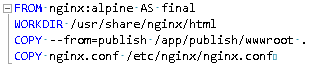
\includegraphics[scale=1]{DockerfileBlazor.png}
	\caption[Screenshot]{Webserver als Basisimage}
\end{figure}

Im Falle einer statischen Website, die von einem \emph{Blazor-WebAssembly}-Projekt erzeugt wird, muss diese zwar mit \emph{.Net} gebaut werden, braucht aber keine \emph{Runtime}-Umgebung, sonder benötigt einen Webserver.
Dies wird wie schon beschrieben erreicht, indem wir die Basis wechseln und die gebauten Daten auf das neue \emph{Basisimage} ziehen, wie auf Abbildung 3.4 gezeigt. Ein Einsprungpunkt wird in diesem Fall nicht benötigt.

Um einen \emph{Dockerfile} nun ausführen zu können und so ein \emph{Image} zu erstellen, müssen wir in der Kommandozeile den Befehl \emph{docker build .} in dem jeweiligen Ordner ausführen. Damit wir das Image später besser referenzieren können, lohnt es sich, dem \emph{Image} ein \emph{Tag} zu geben. Dies machen wir mit dem Kürzel \emph{-t}. Der \emph{Dockerfile} kann mit dem Kürzel \emph{-f} angegeben werden. So kann auch auf eine andere Position in der Ordnerstruktur hingewiesen werden.

Aus Sicherheitsgründen lohnt es sich abzuwägen, ob beim Bauen des \emph{Images} ein neuer Benutzer angelegt und die Anwendung durch diesen gestartet werden sollte. Der Standardnutzer könnte eventuell \emph{Root}-Rechte haben.

\emph{Images} erzeugen zu können ist in Hinblick auf Kubernetes unerlässlich.

\subsubsection{Docker-Compose}

Mithilfe von Docker-Compose lassen sich Container vollständig konfiguriert und durch das Ausführen eines einzelnen Dokumentes starten. Das ermöglicht dem Nutzer komplexe Anwendungssysteme mit nur einem simplen Befehl ausführen zu können. 

\begin{figure}[h!]
	\centering
	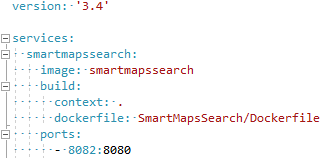
\includegraphics[scale=1]{DockerComposeMin.png}
	\caption[Screenshot]{Beispiel für Docker-Compose}
\end{figure}

Dabei ist Docker-Compose sehr simpel aufgebaut und wird mit der Auszeichnungssprache \emph{YAML} spezifiziert. Im Beispiel, das in Abbildung 3.5 zusehen ist, wird ein Container namens \emph{smartmapssearch} definiert, der ein gleichnamiges \emph{Image} benutzt. Es werden weiterhin ein \emph{Port-Mapping} hinzugefügt und Information zum Bauen des \emph{Images} angegeben. Gebaut wird das \emph{Image} wie zuvor mit einem \emph{Dockerfile}, dessen Position und Namen wir angeben. 

Mit Docker-Compose können aber auch \emph{Volumes} und \emph{Netzwerke} hinzugefügt werden, die natürlich auch gleich an Container angebunden werden können.
Containern kann man ebenfalls auch einen Alias hinzufügen, unter dem sie einen anderen Container innerhalb des Netzwerkes finden können. 

In Abbildung 3.6 sehen wir einen Codeauszug, der dies so implementiert. Unter dem Bezeichner \emph{networks} werden alle Informationen des eigenen Netzwerks angegeben. Das deklarierte Netzwerk ist von Typ \emph{bridge}, was bedeutet, dass Anfragen mit einem bestimmten Alias oder dem Containernamen auf die jeweilige IP-Adresse umgeleitet werden. Von diesem Typ ist auch das Standardnetzwerk. Der Netzwerktyp \emph{host}, der nur unter Linux-Systemen auswählbar ist, wird hier vernachlässigt. Nach den Netzwerken werden wie gewohnt die Container definiert. Denen nun noch das Netzwerk und, wenn gewünscht, auch einen Alias hinzugefügt wird. Hier wurde der Dienst namens \emph{smartsearch} mit einem gleichnamigen Alias versehen. Zu beachten ist, dass die erzeugten Containernamen nicht gleich den Servicenamen sind und es ratsam ist, falls benötigt, einen Alias zu setzen.

\begin{figure}[h!]
	\centering
	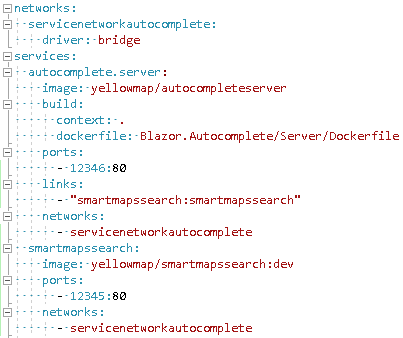
\includegraphics[scale=1]{DockerComposeNetwork.png}
	\caption[Screenshot]{Netzwerk mit Alias}
\end{figure}

\subsection{Praktische Anwendung und Verdikt}

Container sind zusammen mit Docker ein sehr praktisches Werkzeug für die Entwicklung von Diensten. Die isolierte Umgebung, die geboten wird, macht das Entwickeln von kleineren Anwendung  sehr einfach, auch wenn eben diese Isolation anfangs zu so manchen Problemen führt, die zumeist aber durch ein Netzwerk gelöst werden können. In der Praxis war die Containervirtualisierung am besten bei kleineren Anwendungen mit dedizierten Aufgaben zu realisieren, so wie für den Dienst, den ich schon zuvor aus dem Serversystem herauslöste. Durch Docker-Compose ist sogar kleine Ansätze von Skalierbarkeit zu erkennen, doch auch wenn Docker-Compose wesentlich hilft, kleine Systeme aufzubauen und mit anderen Entwicklern zu teilen, ist der Aufwand, der mit der Erhaltung dieses Systems verbunden ist, sehr hoch.

Falls nun in einem Containersystem einer der Container blockieren sollte, muss dies rechtzeitig erkannt werden und der betroffene Container manuell neu gestartet werden. Auch ist \emph{Loging} und \emph{Debugging} sehr umständlich. Dafür muss eine eigene Lösung realisiert werden, die die Logingdaten des Gesamtsystems zum Beispiel in einer Datenbank speichert. In diesem Bereich wäre auch sicherlich eine Lösung mittels Message Broker denkbar.

Die schon angesprochene Skalierbarkeit ist mittels Docker-Compose zu erreichen, aber nur rudimentär implementiert. So lassen sich mit \emph{docker-compose up --scale SERVICE=NUM} eine bestimmte Anzahl an Containern eines bestimmten Dienstes starten. Alternativ kann auch \emph{docker-compose scale SERVICE=NUM} eingesetzt werden. Dieser Befehl gilt aber als veraltet und soll nicht mehr verwendet werden. Hat man innerhalb der \emph{docker-compose.yaml} ein \emph{Port-Mapping} festgelegt, schlägt das Erstellen der Container auch fehl, da diese nicht alle unter demselben Port erreichbar seinen können.


\newpage
\section{Skalierung mit Kubernetes} \label{kubernetes}

Kubernetes ist ein Werkzeug zur Container-Orchestrierung im Besonderen zum Erzeugen und verwalten von Containerclustern. Mit Hilfe von Kubernetes können große, komplexe Containersysteme aufgespannt werden, in denen die einzelnen Anwendungen auf keinen bestimmten Ausführungsort angewiesen sind und es dadurch egal wird, auf welchem Rechner die Anwendungen ausgeführt werden. Neben dem \emph{Routing} übernimmt Kubernetes auch das \emph{Monitoring} der Anwendungen und startet diese neu, wenn diese nicht mehr wie gewohnt zu erreichen sind. Letztlich lässt sich mit Kubernetes auch die Skalierung der Anwendungen automatisieren. Wozu verschiedenste Metriken hinzugezogen werden können. 

\subsection{Kubernetes Komponenten}

Ein Cluster besteht dabei aus mindestens einem Worker-Knoten und einem Master-Knoten. Auf dem Worker-Knoten laufen sogenannte \emph{Pods}, die die Funktion des eigentlichen Containers darstellen. 

\begin{figure}[h!]
	\centering
	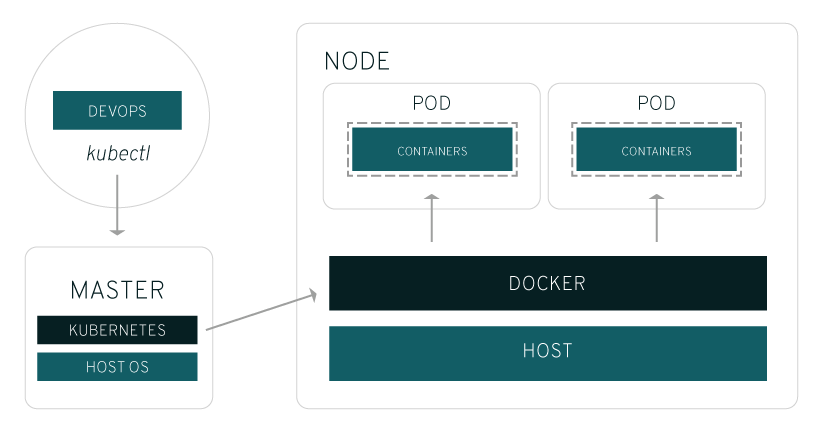
\includegraphics[scale=0.5]{KubeSimpleCluster.png}
	\caption[https://www.redhat.com/de/topics/containers/what-is-kubernetes]{Simples Kubernetes Cluster}
\end{figure}

Auf Abbildung 4.1 sehen wir ein \emph{Kubernetes-Cluster} mit einem \emph{Worker-Knoten} auf dem sich zwei \emph{Pods} befinden. Auf dem \emph{Master-Knoten} laufen alle Controller, die Kubernetes für die Interaktion mit den \emph{Cluster}-Komponenten benötigt. Darunter ist der \emph{API-Server}. Er ist verantwortlich für den allgemeinen Datenaustausch innerhalb des Systems und bietet eine Schnittstelle, über die der Nutzer den Status des \emph{Clusters} abfragen kann, aber die auch allen Komponenten innerhalb des \emph{Clusters} ermöglicht, miteinander zu kommunizieren. Auch werden durch diese Schnittstelle die einzelnen Komponenten konfiguriert.

Mit einem \emph{Worker-Knoten} kommuniziert der \textit{API-Server} über ein \emph{kubelet}, das auf jedem \emph{Worker-Knoten} läuft. Es ist dafür verantwortlich, die auf dem Knoten befindlichen Komponenten zu konfigurieren und zu überwachen. 

\emph{Pods} stellen, wie schon zuvor erwähnt, unsere eigentliche Anwendung dar. Sie werden mit einem Docker-Image konfiguriert und können entweder manuell in der Kommandozeile, mit \emph{YAML} oder automatisch mit einem \emph{Deployment} erzeugt werden. Sie können mehrere Container beinhalten.
Ein \emph{Deployment} ist zur Verwaltung eines \emph{Pods} und seines \emph{ReplicaSets} gedacht. Erstellt man ein \emph{Deployment}, so werden beide Komponenten erzeugt.
Das \emph{ReplicaSet} ist für den Erhalt einer konstanten Anzahl gleichartiger \emph{Pods} gedacht. 
Neben dem \emph{Deployment} gibt es auch \emph{DaemonSets} und \emph{StatefulSets}, die diesem ähneln. 
Ein \emph{DaemonSet} geht sicher, dass auf allen oder auch nur manchen Knoten ein Exemplar des spezifizierten \emph{Pods} läuft. 
Das \emph{StatefulSet} dem entgegen, verhält sich fast wie ein \emph{Deployment}, aber die \emph{Pods}, die es erzeugt, sind nicht absolut austauschbar und besitzen deshalb eine \emph{ID}, mit der man diese auseinanderhalten kann. Dies kann wichtig sein, falls ein Container eigenen Speicher besitzt. 
Egal wie man nun seine \emph{Pods} erzeugt, um auf seine Anwendung zugreifen zu können, braucht man einen \emph{Service}, der einen einfachen Weg bietet, die Anwendung zu erreichen. Auch benötigt man einen \emph{Service}, weil \emph{Pods} innerhalb eines \emph{Deployments} nicht permanent gleich bleiben. Sie werden je nach Bedarf gestartet und beendet und jeder Neue bekommt auch eine neue IP-Adresse zugewiesen. Man kann also die \emph{Pods} auf einem \emph{Deployment} besser erreichen, indem man einen \emph{Service} erzeugt, der alle \emph{Pods} durch eine IP-Adresse erreichbar macht. Eine IP-Adresse lässt sich innerhalb des Clusters aber, ähnlich wie auch Docker, komplett vermeiden, indem man dem Schema \emph{service-name.namespace.svc} folgt.

Mit dem \emph{Cluster} interagieren wir mittels des \emph{kubectl} Befehls. So können wir durch \emph{kubectl create deployment somename --image some/image:test} ein \emph{Deployment} erschaffen und mit \emph{kubectl delete deployment somename} wieder entfernen. 

Doch deutlich genauer und auch angenehmer ist das Erzeugen der Komponenten über \emph{YAML}. 

\begin{figure}[h!]
	\centering
	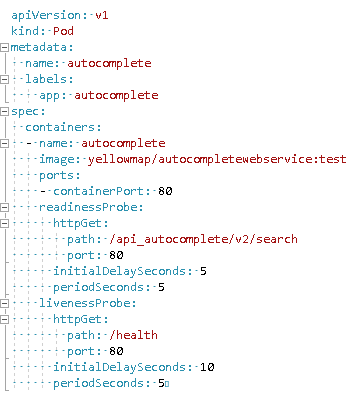
\includegraphics[scale=1]{KubeYmlPod.png}
	\caption[Screenshot]{Pod-Konfiguration YAML}
\end{figure}

Auf der Abbildung 4.2 sehen wir ein Beispiel dazu, wie dies für einen \emph{Pod} aussieht. Zu Beginn wird die \emph{apiVersion}, die Art der Komponente, der Namen und die Labels des \emph{Pods} festgelegt. Die \emph{apiVersion} kann sich von Komponente zu Komponente unterscheiden, wie wir später sehen werden. In \emph{spec} werden nun die zum \emph{Pod} gehörigen Container spezifiziert. Der Unterpunkt \emph{containers} ist eine Liste und kann mehrere Container beinhalten. Zu einem Container gehören Name, Image, eine Liste an Ports und idealerweise auch eine \emph{readinessPobe} und \emph{livenessProbe}. Diese sind in Syntax und Argumenten identisch und unterscheiden sich nur in Funktion. Die \emph{readinessProbe} hat die Aufgabe zu erkennen, ab wann die Anwendung betriebsbereit ist und Anfragen entgegennehmen kann. Die \emph{livenessProbe} überprüft, ob die Anwendung noch betriebsbereit ist oder ob diese neu gestartet werden müsste. Im Beispiel benutzen beide eine HTTP-Anfrage, aber es diese Überprüfung kann auch auf andere Weise realisiert werden.

\begin{figure}[h!]
	\centering
	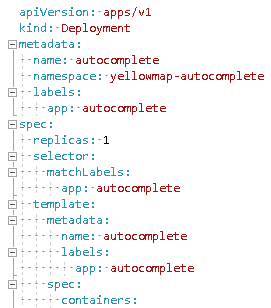
\includegraphics[scale=1]{KubeYmlDep.png}
	\caption[Screenshot]{Deployment-Konfiguration YAML}
\end{figure}

Bei einem \emph{Deployment} verändert sich nur wenig, wie man in Abbildung 4.3 sehen kann. In \emph{metadata} wurde lediglich, um die Komponenten vom Rest des Clusters zu trennen, ein \emph{Namespace} hinzugefügt. In \emph{spec} kommt nun doch mehr hinzu. So können wir nun mit \emph{replicas} die Anzahl der \emph{Pods} in unserem \emph{Deployment} auswählen und mit \emph{selector} werden die vom \emph{Deployment} betroffenen Container ausgewählt. Unter \emph{template} finden wir die \emph{metadata} und \emph{spec} unseres \emph{Pods} aus Abbildung 4.2 wieder.

\begin{figure}[h!]
	\centering
	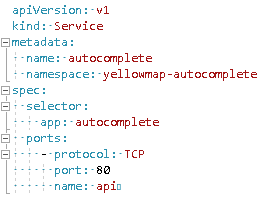
\includegraphics[scale=1]{KubeYmlSvc.png}
	\caption[Screenshot]{Service-Konfiguration YAML}
\end{figure}

Auf Abbildung 4.4 sehen wir zu guter Letzt einen \emph{Service}, der auf diese Weise definiert wird. Die allgemeine Struktur bleibt im Vergleich zu dem \emph{Pod} und dem \emph{Deployment} gleich. In \emph{spec} haben wir einen \emph{selector}, der das \emph{Deployment} referenziert. Danach folgt eine Liste an Ports. Diese werden später dann nach außen zur Verfügung gestellt.

\subsubsection{Helm}

Helm ist eine Erweiterung auf das uns schon bekannte \emph{YAML}-Format, das bei der Erzeugung von Kubernetes-Komponenten zum Einsatz kam. Ein sogenanntes Helm-Chart definiert alle Komponenten im selben Schema wie schon zuvor, doch fügt einiges an Funktionalität hinzu. Ein Helm-\emph{Chart} besitzt eine \emph{Chart.yaml}, die Informationen zum \emph{Chart} beinhaltet, einen \emph{Template}-Ordner, der die \emph{YAML}-Dateien der Komponenten beinhaltet, und eine \emph{values.yaml}, in der Werte global für das komplette Chart gesetzt werden, die dann in den \emph{YAML}-Dateien referenziert werden können. Es können sich auch in einem Charts-Ordner weitere \emph{Subcharts} befinden. Helm-\emph{Charts} können wie auch Images in Registries gespeichert werden.

\subsubsection{Skalierung} 

Die Idee hinter der Skalierung von Prozessen ist es, bei ansteigender Last auf ein System, dies auszugleichen, indem die relevanten Komponenten durch die Zuweisung von Ressourcen oder die Vervielfältigung dieser gestärkt werden.
Die Zuweisung zusätzlicher Ressourcen nennt man vertikale Skalierung, die Vervielfältigung der betroffenen Container horizontale Skalierung.

Beide Arten können durch Kubernetes dynamisch angepasst werden. Dies funktioniert auch automatisch. Bei horizontaler Skalierung erzeugt man in Kubernetes einen \emph{Horizontal Pod Autoscaler (HPA)} auf das gewünschte \emph{Deployment}. Im \emph{Deployment} müssen die Bedingungen für die Replikation der \emph{Pods} angegeben sein. Dies geht am einfachsten über die Angabe der Prozessorauslastung. Zum Lesen der Metrikdaten von \emph{Pods} benötigen wir einen \emph{metrics-server}. Diesen bekommen wir von \emph{Kubernetes SIGs} auf \emph{GitHub}.

\subsection{Aufsetzen eines verteilten Systems}

Nun galt es, das Gelernte in einem weiteren Prototyp zu verwirklichen. Das Ziel war es, das neue Projekt \emph{Autocomplete} mit Testanwendung auf einem Kubernetes-Cluster als ein verteiltes System zu realisieren. Die Testanwendungen waren einerseits eine Benutzeroberfläche zum Testen der Rückgabe auf Nutzereingaben, andererseits ein Dienst zum schreiben von Fehlerberichten auf eine externe Datenbank.
Den Projekten musste jeweils \emph{readiness}- und \emph{liveness}-Endpunkte hinzugefügt werden. Dies macht man in der \emph{Setup.cs} indem man ihn in der Methode \emph{Configure} über \emph{UseEndpoints} konfiguriert. 

\begin{figure}[h!]
	\centering
	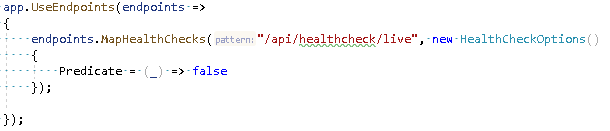
\includegraphics[scale=1]{CsEndpoint.png}
	\caption[Screenshot]{Endpunkte hinzufügen in ASP.NET Core}
\end{figure}

In Abbildung 4.5 wird so ein Endpunkt hinzugefügt, der aber keine \emph{Health Checks} prüft und somit immer \emph{healthy} zurückgeben wird. \emph{Health Checks} werden hier aber nicht weiter betrachtet, da der Fokus der Betrachtung auf Kubernetes liegen soll.

Weiter habe ich für alle betroffenen Projekte mit einem \emph{Dockerfile} Images gebaut und auf eine Registry geschoben, auf die ich von dem Cluster aus Zugriff hatte. Die Adressen der Dienste, die nun innerhalb des Clusters laufen und untereinander kommunizieren sollten, mussten davor natürlich so angepasst werden, dass diese auf einen \emph{Service} und nicht einfach auf eine Adresse oder auf einen Container verwiesen. Kleinere Probleme gab es mit der \emph{Registry}, da diese eine \emph{insecure registry} war und somit dem Cluster hinzugefügt werden musste.

Um ein \emph{Cluster} auf dem eigenen Rechner aufzusetzen, eignet sich Minikube. Wurde Minikube installiert und den Umgebungsvariablen hinzugefügt, können wir mit \emph{minikube start} ein eigenes \emph{Cluster} starten. Das ist sinnvoll aus Test- und Entwicklungszwecken. Mit Minikube lässt sich die Verwendung eines \emph{Ingress}-Controllers komplett vermeiden. Ein \emph{Service} kann auf \emph{localhost} erreicht werden, wenn dieser mit \emph{minikube service svc-name} ausgeführt wird. 

Nachdem ich die Funktion vorerst lokal getestet hatte, konnte ich nun anfangen, die verschiedenen \emph{YAML}-Dateien für die Kuberntes-Komponenten zu schreiben. Diese blieben zumeist unverändert von den Testdateien, die ich schon zuvor erstellt hatte. Für die drei Anwendungen gab es jeweils ein \emph{Deployment} und einen \emph{Service}. Des Weiteren gab es einen \emph{Ingress}, der Anfragen auf die drei \emph{Services} aufteilt. Ich verwendete \emph{livenessProbes} und \emph{readinessProbes} aber musste leider die automatische Skalierung außer acht lassen, da der \emph{metrics-server} weder auf dem Testsystem vorhanden war, noch ich die nötigen Rechte hatte, ihn zu installieren. Für den Gebrauch der \emph{Registry} musste ein \emph{Secret} auf dieser hinzugefügt werden. Ebenso musste das \emph{Secret} in der Datei unter \emph{imagePullSecrets} referenziert werden. Da das Image, wenn sich dessen Namen oder \emph{Tag} nicht verändert hat, nicht aktualisiert und die lokale Version verwendet wird, setzte ich die \emph{imagePullPolicy} auf \emph{Always}.

\begin{figure}[h!]
	\centering
	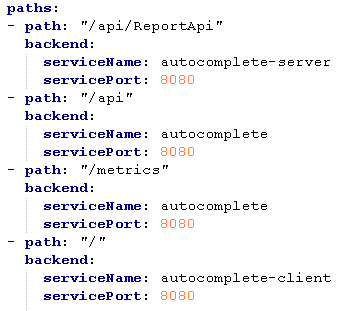
\includegraphics[scale=1]{KubeIngressPaths.png}
	\caption[Screenshot]{Ingress Paths}
\end{figure}

Auf Abbildung 4.6 sehen wir, unter welchen Paths die verschiedenen Services durch den Ingress erreichbar sind. Interessant ist, dass aufgepasst werden muss, dass Anwendungen sich mit ihren Endpunkten nicht gegenseitig in die Quere kommen, falls wir wollen, dass diese auf derselben URL erreichbar sind. 
Somit interagieren wir mit den Containern, als wären diese ein einzelnes System, aber halten diese austauschbar und dynamisch.

Ein Helm-Chart erstellte ich nur für die \emph{Autocomplete}-Anwendung, für die Testanwendungen war dies meiner Meinung nicht notwendig, da diese nur zum Testen benötigt wurden.


\newpage
\section{Fazit}\label{conclusion}
Nach Abschluss der Arbeit gilt nun zu bewerten, ob und wie die gesetzten Vorgaben denn jetzt schließlich erreicht oder auch nicht erreicht wurden.

Dazu vorerst einen kleinen Rückblick auf das Geschaffene. Das Produkt der Arbeit sind zweit funktionstüchtige Prototypen. Diese resultieren einmal aus der Untersuchung zur Nachrichtenübermittlung mittels Message Broker und der Untersuchung zur Containervirtualisierung und Containerorchestrierung. 

Die Untersuchung der Nachrichtenübermittlung mittels Message Broker, die mit RabbitMQ durchgeführt wurde, sollte eine dynamische Kommunikation zwischen den sonst unabhängigen Anwendungen schaffen. Dies wurde auch ermöglicht und funktionierte zuverlässig, aber die spätere Untersuchung zur Containerorchestrierung bot ebenfalls gute Wege zur dynamischen Kommunikation zwischen den verschiedenen Anwendungen innerhalb des Clusters. Ein finales Verdikt hierzu sollte durch eine weitere Untersuchung in Betracht gezogen werden. Nichtsdestotrotz bot RabbitMQ, durch die Funktion eine Nachricht an viele Konsumenten auf einmal zu verteilen, einen Mehrwert, der im Sammeln von \emph{Logging}-Daten weiter Verwendung finden kann.

Die Untersuchung zur Containervirtualisierung, die mit Docker durchgeführt wurde, sollte Anwendungen eine Umgebung zur Verfügung stellen, in der sie unabhängig von anderen Anwendungen und deren Abhängigkeiten ausgeführt werden können. Dies war ebenfalls erfolgreich, aber ebenfalls soll angemerkt sein, dass die Notwendigkeit einer Nachuntersuchung zur Fehlersuche und \emph{Logging} bezüglich Containern in Betracht gezogen werden sollte, da dies hier nur in der Essenz betrachtet wurde.

Die Untersuchung zur Containerorchestrierung, die mit Kubernetes durchgeführt wurde, baute auf der vorherigen Untersuchung zur Containervirtualisierung auf und sollte eine Umgebung bieten, in der die zuvor untersuchten Container auf verschiedenen Systemen als ein System laufen können. Auch sollte untersucht werden, wie die einzelnen Container von Kubernetes überwacht und neu gestartet werden können. Dies wurde zufriedenstellend erreicht. Weitere Folgeuntersuchungen, die in Betracht gezogen werden könnten, wären hierzu ebenfalls zur Fehlersuche und \emph{Logging}, aber auch wäre eine Untersuchung zur Skalierbarkeit denkbar.

Nun zur Betrachtung der Arbeit an Hand der drei gesetzten Begriffen der Flexibilität, Unabhängigkeit und Robustheit.
Die Flexibilität wird auf vielerlei Weise erreicht. Durch die Möglichkeiten über einen Message Broker oder auch über das in Kubernetes enthaltene \emph{Routing} gibt uns die Freiheit, Anwendungen auszutauschen, ohne mit direkten Adressen zu tun zu haben, das heißt, wenn eine neue Anwendung mit neuer Adresse startet, wird diese trotzdem wie zuvor erreicht. 

Die Unabhängigkeit wird durch die Containervirtualisierung erreicht, die den Anwendungen eigene Umgebung bietet, in der jede Anwendung durch den Container, in dem sie läuft, abgeschirmt von äußeren Einflüssen ist.

Die Robustheit wird durch Kubernetes erreicht. Kubernetes ist in der Lage, durch die \emph{livenessProbe} und die \emph{readinessProbe} zu erkennen, ob ein Container noch wie gewünscht antwortet und startet diesen neu, falls dies nicht der Fall sein sollte. Somit können Container nicht nur bei einem Absturz, sondern auch bei internen Fehlern automatisch neu gestartet werden.

Somit wurden alle drei Begriffe erfüllt und damit das Forschungsprojekt erfolgreich abgeschlossen.

%Und jetzt spitzt das warme Blut aus dem Hals der letzten Sau. Und mit ihr stirbt ein kleines Stück Geschichte unserer Stadt. Der Sau ist es egal, doch wir wissen es genau. Der Bagger macht viel mehr als nur den alten Schlachthof platt. 
%Ich bin mir nicht sicher aber eines weis ich genau. Tote tanzen keinen Pogo, trinken keinen Alkohol. Tote nehmen keine Drogen. Auch ohne Rausch fühlen sie sich wohl.
%Und du bist schuldig weil du Hausbesetzer bist. Du hast kein Geld und keinen Job und grüne Haare auf'm Kopf. Die scheiß Gesellschaft mach dich krank. Du bist ein Punk.

\newpage

%--------------------------------
% Ab hier => Literaturverzeichnis
%--------------------------------

\printbibliography
\addcontentsline{toc}{section}{Literaturverzeichnis}
\end{document}